\documentclass[a4paper,10pt,twoside,openany]{book}

\usepackage[lang=hebrew]{maths}
\usepackage{hebrewdoc}
\usepackage{stylish}
\usepackage{lipsum}

\title{סיכומי הרצאות ביריעות דיפרנציאביליות \\ \large{חורף 2018, הטכניון}}
\author{הרצאותיו של מיכאל חנבסקי \\ \large סוכמו על ידי אלעד צורני}
\date{\today}

\begin{document}
\frontmatter
\frontpage{atlas}{0.8\textwidth}{מפת העולם. על ידי ג'ררד ואן שגן.}
\tableofcontents
\countlectures
\newpage

\chapter*{הקדמה}
\addcontentsline{toc}{chapter}{הקדמה} \markboth{הקדמה}{}

\section*{הבהרה}
\addcontentsline{toc}{section}{הבהרה} %\markboth{Technicalities}{}

סיכומי הרצאות אלו אינם רשמיים ולכן אין
\emph{כל הבטחה}
כי החומר המוקלד הינו בהתאמה כלשהי עם דרישות הקורס, או שהינו חסר טעויות.
\\
להיפך, ודאי ישנן טעויות בסיכום! אעריך אם הערות ותיקונים ישלחו אלי בכתובת דוא"ל
\textenglish{\href{mailto:tzorani.elad@gmail.com}{tzorani.elad@gmail.com}}.\\
אלעד צורני.

\section*{ספרות מומלצת.}
\addcontentsline{toc}{section}{ספרות מומלצת} %\markboth{Course Literature}{}

הספרות המומלצת עבור הקורס הינה כדלהלן.

\begin{english}
\begin{description}
\item[M. Spivak:] Calculus on manifolds: a modern approach to classical theorems of advanced calculus

\item[J. Milnor:] Topology from athe differentiable viewpoint

\item[J. Lee:] Introduction to smooth manifolds

\item[L. Conlon:] Differentiable manifolds: a first course

\item[V. Guillemin, A, Pollcak:] Differential topology
\end{description}
\end{english}

\mainmatter

\chapter*{הקדמה}
\section{תוכן הקורס}
\stress{יריעה}
היא מרחב טופולוגי שלוקלית נראה כמו קבוצה פתוחה ב־%
$\RR^n$.%
\newlecture{21 באוקטובר}{2018}
דוגמאות ליריעות הן עקומות ומשטחים.
\begin{example}
$S^2$
הינה יריעה. סביבה של נקודה נראית כמו קבוצה פתוחה ב־%
$\RR^2$.
\end{example}
\begin{example}
$\TT^2$
הינה יריעה. סביבה של נקודה גם כאן נראית כמו קבוצה פתוחה ב־%
$\RR^2$.
\end{example}
נסתכל על העתקה
$f \colon S^2 \to \TT^2$.
נוכל לזהות את ההעתקה
$f \colon \RR^2 \to \RR^2$
באופן לוקלי עם העתקה
$\hat{f}$
שמעתיקה קבוצות פתוחות לקבוצות פתוחות. ראו איור
\ref{fig1}.
\begin{figure}[ht]
\centering
\caption{העתקה לוקלית.}
\label{fig1}
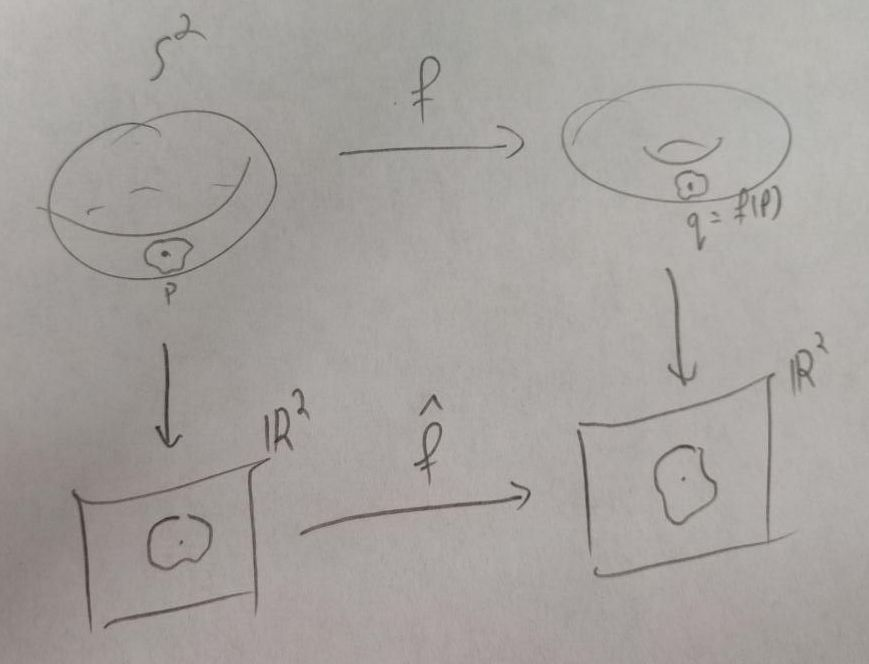
\includegraphics[width=0.8\textwidth]{sources/figure1}
\end{figure}
\\
בקורס נעסוק בהכללת משפטים מאנליזה ב־%
$\RR^n$
למשפטים על יריעות חלקות.
רוב המשפטים ניתנים להכללה ליריעות $\CCC^k$.
למשפטים מהקורס שימושים רבים בגיאומטריה, טופולוגיה, פיזיקה, אנליזה, קומבינטוריקה ואלגברה. כדי שהתיאוריה הקשורה לקורס לא תישאר באוויר נראה חלק גדול מהקורס שימושים, בעיקר בתחום של טופולוגיה דיפרנציאלית.
\\
קיימים מספר משפטים מוכרים מאנליזה.
\\
\begin{examples}
\begin{enumerate}
\item \emph{נוסחאת ניוטון-לייבניץ:}
\[\int_{\del\brs{a,b}} F = \int_{\brs{a,b}} F' \diff x\]
\item \emph{נוסחאת גרין:}
\[\int_{\del U} f\diff x + g \diff y = \iint_{U} \prs{\frac{\del g}{\del x} - \frac{\del f}{\del{y}}} \diff x \diff y\]
\item \emph{משפט גאוס:}
\[\iiint_{\Omega} \div \vec{F} \diff v = \iint_{\del \Omega} \trs{\vec{F},\vec{n}} \diff s\]
\item \emph{משפט סטוקס:}
\[\iint_{\Sigma} \trs{\rot \vec{F}, \vec{n}} \diff s = \int_{\del \Sigma} \trs{\vec{F}, \vec{\gamma}} \diff t\]
\end{enumerate}
\end{examples}
כולם נובעים ממשפט סטוקס כללי יותר אותו נוכיח בקורס.
\[\int_{\del \Omega} \omega = \int_{\Omega} \diff \omega\]

\section{דרישות קדם}
נשתמש בקורס רבות במשפט הפונקציה הסתמונה ובמשפט הפונקציה ההפוכה מ־%
$\RR^n$.
רצוי להכיר את ניסוחיהם, את המשמעויות הגיאומטריות ומספר שימושים שלהם.
נשתמש בהחלפות קואורדינטות מאלגברה לינאריות, במשפט פוביני, מטריצות יעקוביאן, במטריצות יעקוביאן, בכלל השרשרת ובמשפט קיום ויחידות של מד"ר.

\section{תרגילי בית}
בקורס יפורסמו ארבעה תרגילי בית רשמיים, רובם ברמת הבנת ההגדרות. אין חובת הגשה אך מומלץ מאוד לפתור את התרגילים כדי לוודא שאינכם הולכים לאיבוד.

\section{ציון}
הציון הסופי כולו יסתמך על הגשת עבודת בית.

\chapter{מבוא}
\section{הגדרות}
\begin{definition}
מרחב טופולוגי
$M$
נקרא
\stress{יריעה טופולוגית}
\textenglish{(topological manifold)}
אם לכל
$x \in M$
יש סביבה
$U$
שהומאומורפית לקבוצה פתוחה ב־%
$\RR^n$
עבור
$n$
כלשהו.
\end{definition}
\begin{remark}
לעתים יריעה טופולוגית כפי שהגדרנו אותה נקראת
\stress{מרחב אוקלידית לוקלית}
\textenglish{locally Euclidean space}.
\end{remark}
\begin{fact}
עבור יריעה טופולוגית,
$n$
קבוע מקומית.
\\
אם
$M$
קשירה,
$n$
קבוע.
\end{fact}
\begin{definition}
עבור יריעה
$M$
עם
$n$
קבוע, נגיד ש־%
$n$
הוא
\stress{המימד}
של היריעה.
\end{definition}
\begin{exercise}
מצאו אילו אותיות מבין
\textenglish{MANIFOLD}
הן יריעות. מצאו אילו הומאומורפיות.
\end{exercise}
\begin{examples}
\begin{enumerate}
\item עקומות
\item משטח ב־%
$\RR^3$
\item $S^n \subseteq \RR^{n+1}$:
נסמן
$\Uu^+ = S^n \setminus \set{p^+}$
נתאים לנקודה
$x \in \Uu^+$
על הספירה את הנקודה
$\phi^{+}(x) \in \RR^n$
המתקבלת על ידי הטלה סטרוגרפית. ראו איור
\ref{fig2}.
\begin{figure}[ht]
\centering
\caption{הטלה סטרוגרפית.}
\label{fig2}
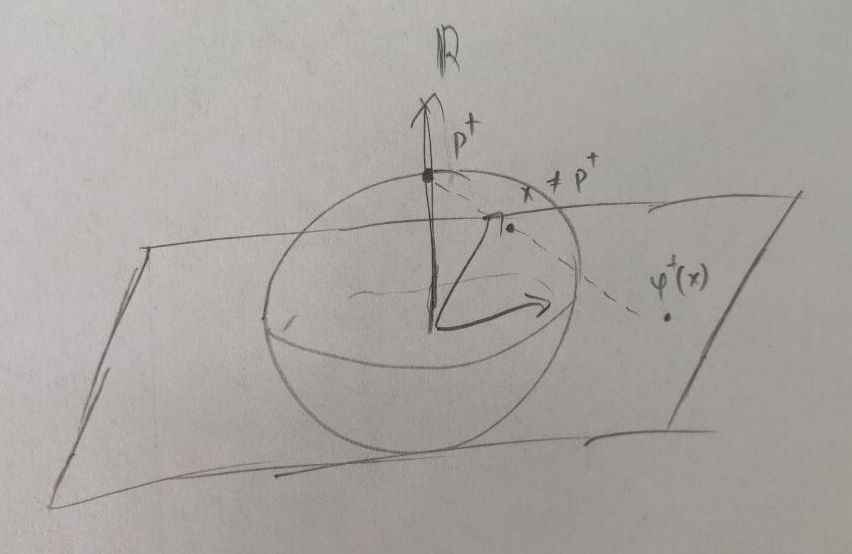
\includegraphics[width=0.8\textwidth]{sources/figure2}
\end{figure}
ניתן לראות כי
$\phi^+$
הומאומורפיזם.
אפשר באותו אופן להגדיר
$\phi^{-} \colon \U^{-} \to \RR^n$.
לכל נקודה על
$S^n$
יש סביבה הומאומורפית לקבוצה פתוחה ב־%
$\RR^n$
המתקבלת מהמקור דרך
$\phi^{\pm}$
של סביבה בתמונה, לכן
$S^n$
יריעה.
\end{enumerate}
\end{examples}
\begin{exercise}
אם
$M_1, M_2$
יריעות טופולוגיות אז
$M_1 \times M_2$
עם טופולוגיית המכפלה הינה יריעה.
אם המימד של
$M_1, M_2$
אחיד מתקיים גם
\[\text{.} \dim\prs{M_1 \times M_2} = \dim{M_1} + \dim{M_2}\]
\end{exercise}
\begin{example}
\stress{טורוס
$n$–%
מימדי} הוא
$\TT^n \ceq \prod_{k=1}^n S^1$.
ניתן להגדיר גם
$T^n = \quot{\RR^n}{\ZZ^n} = \quot{\RR^n}{\sim}$
כאשר
$x \sim y$
אם
$x-y \in \ZZ^n$.
נסמן
$\pi \colon \RR^n \to T^n$
את ההטלה הטבעית (כלומר
$\pi\prs{x} = \brs{x} = x+\ZZ^n$)
ואז
$\Uu \subseteq T^n$
פתוחה אם
$\pi^{-1}\prs{\Uu}$
פתוחה ב־%
$\RR^n$.
\end{example}
\begin{exercise}
הראו כי
$\TT^n$
הומאומורפי ל־%
$T^n$.
\end{exercise}
\begin{example}
נגדיר
\stress{מרחב פרויקטיבי הוא}
בשתי דרכים.
\begin{enumerate}[label = (\roman*)]
\item
נסתכל על ישרים דרך
$\vec{0}$
ב־%
$\RR^{n-1}$.
עבור
$\ell$
ישר דרך
$0$
נסמן
$\Uu_{\eps}\prs{\ell}$
את אוסף הישרים
$\ell'$
דרך
$\vec{0}$
כך שמתקיים
$\deg{\ell, \ell'} < \eps$.
אז קבוצה פתוחה היא איחוד כלשהו של
$\Uu_{i\in I} \Uu_{\eps_i}\prs{\ell_i}$.
\item
נגדיר גם
$RP^n = \quot{S^n}{\pm 1}$
כלומר
$x \sim y$
אם
$x = \pm y$.
נסמן
$\pi \colon S^n \to RP^n$
את ההטלה
$x \to \set{x, -x}$
ואז
$\Uu \subseteq RP^n$
פתוחה אם
$\pi^{-1}\prs{\Uu}$
פתוחה ב־%
$\S^n$.
\end{enumerate}
\end{example}
\begin{exercise}
הראו כי
$\R P^n$
הומאומורפי ל־%
$RP^n$.
\end{exercise}
\begin{example}
$\R P^1$
הומאומורפי ל־%
$\S^1$.
לאחר הזיהוי מתקבל קטע המזוהה בקצותיו, וזה הומאומורפי למעגל.
\end{example}
\begin{definition}
תהי
$M$
יריעה טופולוגית.
\stress{מפה}
\textenglish{map / coordinate chart}
היא זוג
$\prs{\Uu, \phi}$
כאשר
$\Uu \subseteq M$
קבוצה פתוחה ו־%
$\phi \colon \Uu \to \phi(\Uu) \subseteq \RR^n$
הומאומורפיזם, ו־%
$\phi\prs{\Uu} \subseteq \RR^n$
פתוחה.
\end{definition}
\begin{example}
ב־%
$S^n$
הגדרנו שתי מפות
$\prs{\Uu^{\pm}, \phi^{\pm}}$.
\end{example}
\begin{definition}
תהיינה
$\prs{\Uu, \phi}, \prs{\Vv, \psi}$
מפות עבור יריעה
$M$.
אז
$\phi \circ \psi^{-1} \colon \psi\prs{\Uu \cap \Vv} \to \phi\prs{\Uu \cap \Vv}$
הומאומורפיזם שנקרא
\stress{פונקציית מעבר} \textenglish{transition map}
או
\stress{פונקציית החלפת קואורדינטות}.
ראו איור
\ref{fig3}
\begin{figure}[ht]
\centering
\caption{פונקציית מעבר.}
\label{fig3}
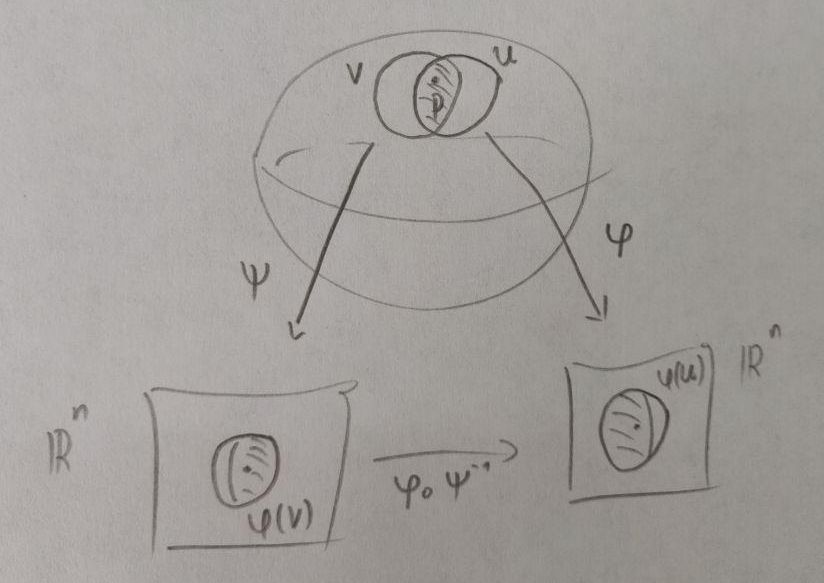
\includegraphics[width=0.8\textwidth]{sources/figure3}
\end{figure}
\end{definition}
\begin{definition}
תהי העתקה
$f \colon M \to N$
בין יריעות, ונניח בה"כ
$f\prs{\Uu_1} \subseteq \Vv_1$.
אז
$\hat{f}_1 \colon \phi_1\prs{\Uu_1} \to \psi_1\prs{\Vv_1}$
\stress{הצגה מקומית של
$f$}
(ביחס למפות
$\prs{\phi_1, \Uu_1}$
ו־%
$\prs{\psi_1, \Vv_1}$).
מתקיים
$\hat{f}_1 = \eval{\psi_1 \circ f \circ \phi_1^{-1}}{\psi_1\prs{\Uu_1}}{}$.
ראו איור
\ref{fig4}.
\begin{figure}[ht]
\centering
\caption{הצגה מקומית.}
\label{fig4}
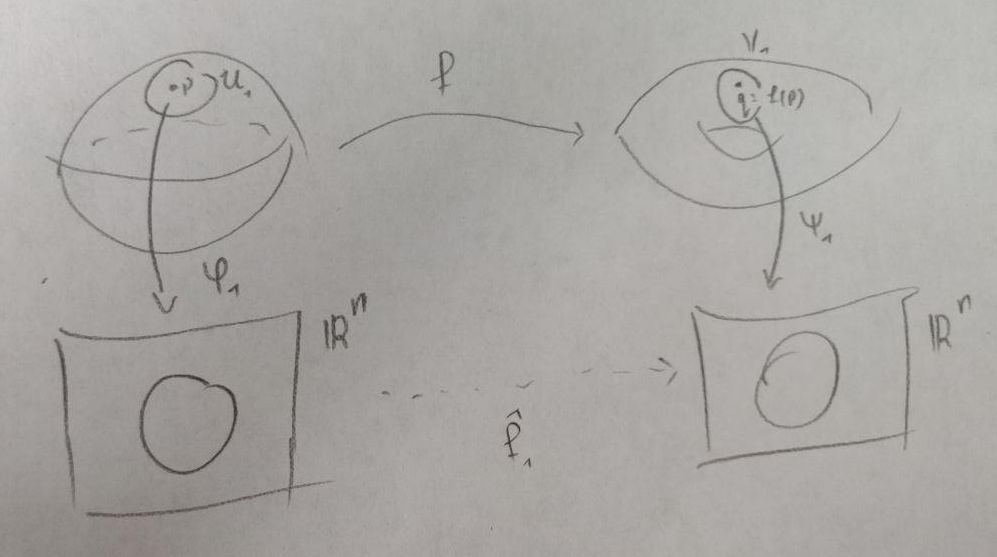
\includegraphics[width=0.8\textwidth]{sources/figure4}
\end{figure}
\end{definition}
\begin{definition}
תהיינה
$\hat{f}_1, \hat{f}_2$
שתי הצגות מקומיות של
$f \colon M \to N$.
אז
\[\text{.} \eval{\hat{f}_2}{\phi_2\prs{\Uu_1 \cap \Uu_2}}{} = \psi_2 \circ \psi_1^{-1} \circ \hat{f}_1 \circ \phi_1 \circ \phi_2^{-1}\]
כאן
$\phi_1 \circ \phi_2^{-1}$
פונקציית מעבר מ־%
$\prs{\Uu_2, \psi_2}$
ל־%
$\prs{\Uu_1, \phi_1}$
ו־%
$\psi_2 \circ \psi_1^{-1}$
פונקציית מעבר מ־%
$\prs{\Vv, \psi_1}$
ל־%
$\prs{\Vv, \psi_2}$.
ראו איור
\ref{fig5}.
\begin{figure}[ht]
\centering
\caption{פונקציית מעבר בין יריעות.}
\label{fig5}
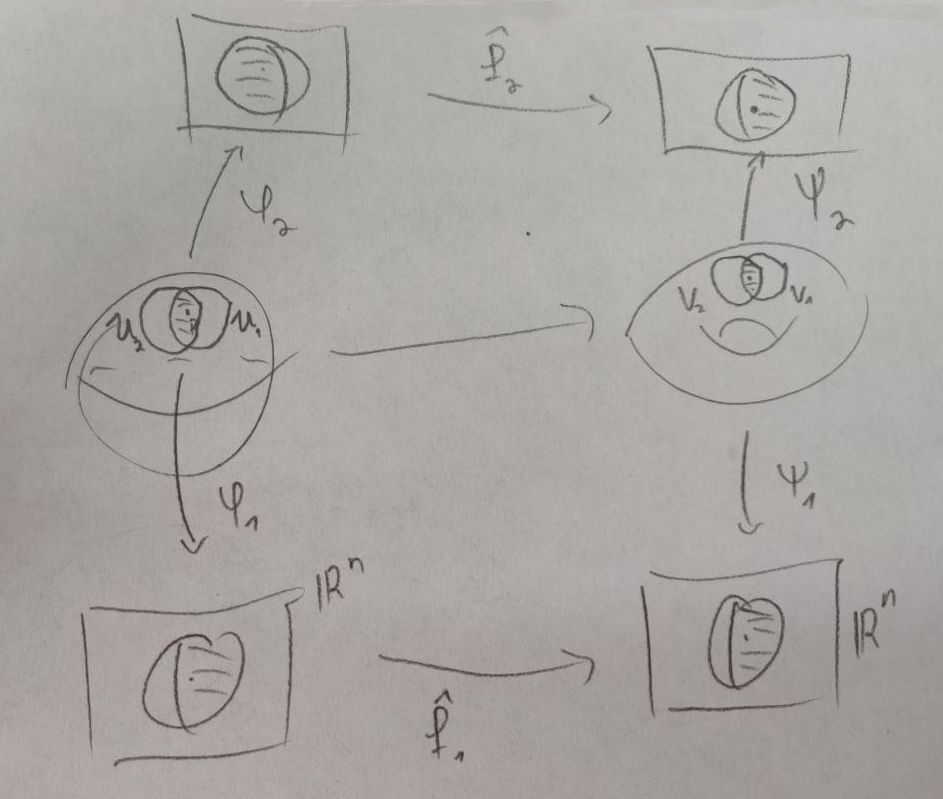
\includegraphics[width=0.8\textwidth]{sources/figure5}
\end{figure}
\end{definition}
נזכיר כי
$f \colon \Uu \to \RR^m$
עבור
$\Uu \subseteq \RR^n$
נקראת
\stress{חלקה}
\textenglish{(smooth)}
אם לכל
$x \in \Uu$
קיימות ורציפות נגזרות חלקיות של
$f$
מסדר כלשהו.
\begin{notation}
עבור
$f$
חלקה נסמן
$f \in \CCC^{\infty}$.
\end{notation}
\begin{definition}
$f \colon \Uu \to \Ww$
עבור
$\Uu \subseteq \RR^n, \Ww \subseteq \RR^m$
\stress{דיפאומורפיזם}
אם
$f$
הפיכה, ו־%
$f,f^{-1}$
חלקות.
\end{definition}
\begin{exercise}
אם
$f \colon \Uu \to \Ww$
חלקה וגם
$\Uu \subseteq \RR^n, \Ww \subseteq \RR^m$
אז
$m=n$.
\end{exercise}
\begin{examples}
\item $f(x) \ceq \fcases{0 & x < 0 \\ x^2 & x \geq 0}$
איננה חלקה.
\item $f(x) \ceq \fcases{0 & x \leq 0 \\ e^{-\frac{1}{x}} & x > 0}$
חלקה (אך איננה אנליטית).
\item נגדיר $\Uu = \prs{-\frac{\pi}{2}, \frac{\pi}{2}}, \Ww = \R$.
אז
$\tan \colon \Uu \to \Ww$
דיפאומורפיזם.
\end{examples}
\begin{exercise}
\begin{enumerate}
\item אם
$F$
דיפאו' גם
$F^{-1}$
דיפאו'.
\item הרכבה של דיפאו' היא דיפאו'.
\item אם
$F_1 \colon \Uu_1 \to \Ww_1$
ו־%
$F_2 \colon \Uu_2 \to \Ww_2$
דיפאו' אז
$F_1 \times F_2 \colon \Uu_1 \times \Uu_2 \to \Ww_1 \to \Ww_2$
דיפאו'.
\item אם
$-\infty \leq a \leq b \leq \infty$
ו־%
$-\infty \leq c \leq d \leq \infty$
אז
$\prs{a,b}$
דיפאומורפי ל־%
$\prs{c,d}$.
\item הקבוצות במישור
מאיור
\ref{fig6}
דיפאומורפיות.
\begin{figure}[ht]
\centering
\caption{קבוצות דיפאומורפיות במישור.}
\label{fig6}
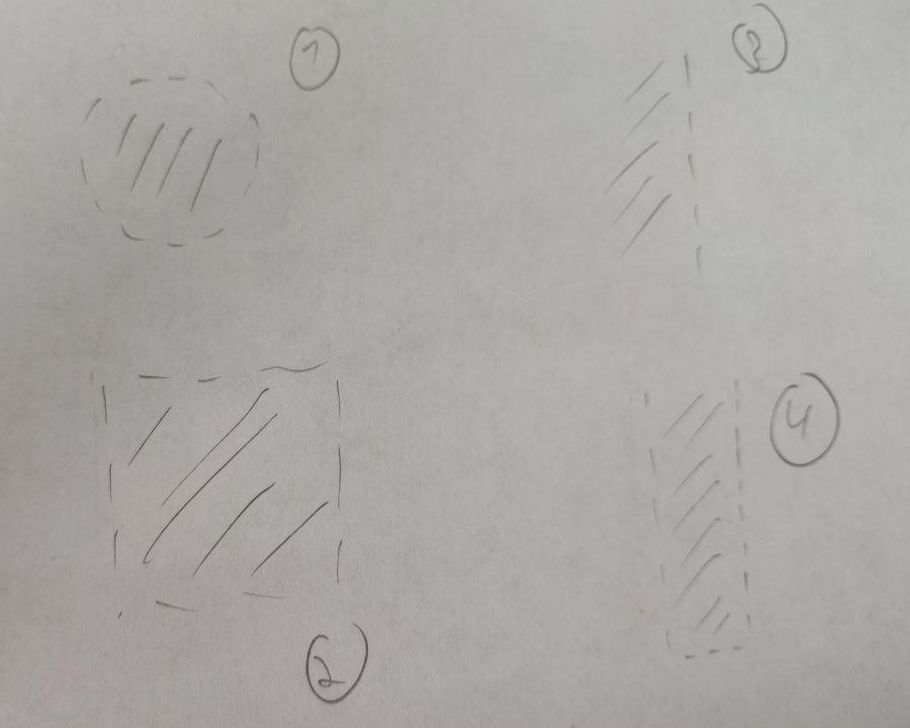
\includegraphics[width=0.8\textwidth]{sources/figure6}
\end{figure}
\end{enumerate}
\end{exercise}
\backmatter
\end{document}

